% !TEX root = ../../../main.tex

\toggletrue{image}
\toggletrue{imagehover}
\chapterimage{x}
\chapterimagetitle{\uppercase{X}}
\chapterimageurl{https://xkcd.com/2309/}
\chapterimagehover{The worst is when you run out of monospaced fonts and have to use variable-width variables.}


\chapter{Variablen}
\label{ch:variablen}

Für einfachere und vielseitigere Programme müssen wir in der Lage sein, einen Integer oder einen String zu speichern. In Python gibt es dafür \textbf{benannte Speicherplätze}. Das Speichern in benannten Speicherplätzen ist nicht zu verwechseln mit dem Speichern z.B.\ eines Textdokuments. Ein Speicherplatz steht nur zur Verfügung, solange das Programm läuft. Danach werden alle Speicherplätze gelöscht. Die Lernziele für dieses Kapitel sind:\\

\lernziel{\autoref{ch:variablen}, \nameref{ch:variablen}}{
\begin{minipage}{\linewidth}
$\square$ \hspace{0.1cm} Sie definieren die Begriffe Variable und Zuweisung.\\
$\square$ \hspace{0.1cm} Sie verwenden Variablen, um Python-Programme einfacher und vielseitiger zu machen.\\
$\square$ \hspace{0.1cm} Sie wissen, welche Variablennamen in Python erlaubt sind.\\
$\square$ \hspace{0.1cm} Sie berücksichtigen die Clean-Code-Regeln im Umgang mit Variablen.
\end{minipage}
}

\section{Quadrate mit unterschiedlicher Länge}
\label{sec:quadrate-mit-unterschiedlicher-laenge}

Betrachten wir das Programm in \autoref{lst:quadrat-100} (Quadrat, Seitenlänge $100$). Wenn wir nun ein Quadrat mit der Seitenlänge $275$ zeichnen wollen, müssen wir das Programm an \textbf{vier} Stellen anpassen. \autoref{lst:quadrat-275} zeigt das angepasste Programm. Optimal wäre es, wenn wir das Programm nur an \textbf{einer} Stelle anpassen müssten. Dies kann durch die Verwendung einer \textbf{Variablen} erreicht werden.

\begin{figure}[htb]
    \centering
    \begin{minipage}{0.4\linewidth}
        \centering
        \begin{lstlisting}[language={python3}, caption={Quadrat (Länge $100$).}, label={lst:quadrat-100}]
import turtle

turtle.fd(100)
turtle.lt(90)
turtle.fd(100)
turtle.lt(90)
turtle.fd(100)
turtle.lt(90)
turtle.fd(100)
turtle.lt(90)
turtle.done()

\end{lstlisting}
\end{minipage}
\hfill
\begin{minipage}{0.4\linewidth}
\centering
\begin{lstlisting}[language={python3}, caption={Quadrat (Länge $275$).}, label={lst:quadrat-275}]
import turtle

turtle.fd(275)
turtle.lt(90)
turtle.fd(275)
turtle.lt(90)
turtle.fd(275)
turtle.lt(90)
turtle.fd(275)
turtle.lt(90)
turtle.done()

\end{lstlisting}
\end{minipage}
\end{figure}

Wir speichern den Integer für die Seitenlänge des Quadrats in einer Variablen ab und verwenden diese Variable dann als Argument für die vier Funktionsaufrufe. \autoref{lst:quadrat-var-100} zeigt das verbesserte Programm. Wenn das Programm ausgeführt wird, dann wird in Zeile \textbf{drei} der Integer $100$ in der Variablen mit dem Namen \lstinline[language={python3}]{a} gespeichert. In den Zeilen vier, sechs, acht und zehn wird die Variable \lstinline[language={python3}]{a} dann durch den gespeicherten Integer, das heisst $100$ ersetzt.

\begin{figure}[htb]
\centering
\begin{minipage}{0.4\linewidth}
\centering
\begin{lstlisting}[language={python3}, caption={Die Variable \texttt{a} speichert den Integer $100$ (\graybgtexttt{quadrat\_var.py}).}, label={lst:quadrat-var-100}]
import turtle

a = 100
turtle.fd(a)
turtle.lt(90)
turtle.fd(a)
turtle.lt(90)
turtle.fd(a)
turtle.lt(90)
turtle.fd(a)
turtle.lt(90)
turtle.done()

\end{lstlisting}
\end{minipage}
\hfill
\begin{minipage}{0.4\linewidth}
\centering
\begin{lstlisting}[language={python3}, caption={Zeile drei wurde angepasst - nun wird der Integer $275$ gespeichert.}, label={lst:quadrat-var-275}]
import turtle

a = 275
turtle.fd(a)
turtle.lt(90)
turtle.fd(a)
turtle.lt(90)
turtle.fd(a)
turtle.lt(90)
turtle.fd(a)
turtle.lt(90)
turtle.done()

\end{lstlisting}
\end{minipage}
\end{figure}

Jetzt können wir das Programm leicht ändern. Wenn wir ein Quadrat mit der Seitenlänge $275$ haben wollen, dann müssen wir nur Zeile drei ändern. \autoref{lst:quadrat-var-275} zeigt das angepasste Programm.

\section{Was ist eine Variable?}
\label{sec:was-ist-eine-variable}

Wir können uns eine Variable als einen Behälter mit einem Etikett vorstellen, in dem ein Wert gespeichert wird. In \autoref{figure:variables-boxes} sind zwei Variablen als Behälter dargestellt.

\begin{figure}[htb]
\centering
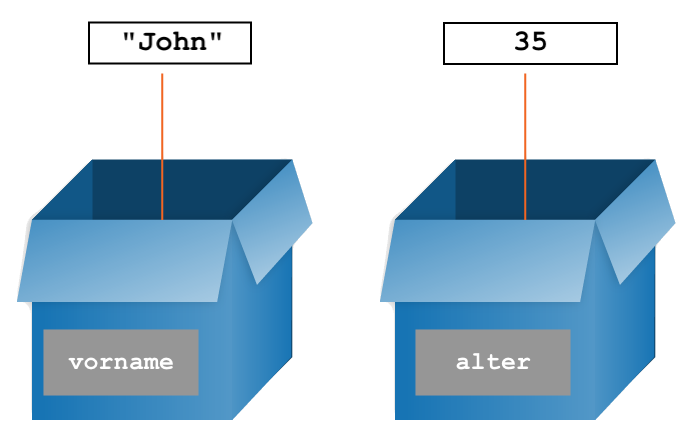
\includegraphics[height=4.25cm]{boxesVariable}
\caption{Zwei Variablen, dargestellt als Behälter mit Etiketten.\protect\footnotemark}
\label{figure:variables-boxes}
\end{figure}

\footnotetext{Bildquelle: Angepasst von \url{http://www.pyworld.in/Python/pythonVariables.html?i=1}.}

Jeder Behälter in \autoref{figure:variables-boxes} hat ein Etikett und einen gespeicherten Wert. Der Behälter mit dem Etikett \lstinline[language={python3}]{vorname} entspricht einer Variablen mit dem Namen \lstinline[language={python3}]{vorname} und dem gespeicherten Wert \lstinline[language={python3}]{"John"} (ein String). Die andere Variable heisst \lstinline[language={python3}]{alter} und speichert den Wert \lstinline[language={python3}]{35} (einen Integer).

\begin{definition}[Variable]
Eine Variable ist ein \textbf{Speicherplatz mit einem Namen}. In der Variablen kann ein \textbf{beliebiger Wert} gespeichert werden. Dies geschieht in Python mit einer \textbf{Zuweisung}. Wir können den gespeicherten Wert auch wieder auslesen. Dazu notieren wir den Namen der Variablen. Den Namen einer Variablen können wir selbst wählen.
\end{definition}

\section{Was ist ein Wert?}
\label{sec:was-ist-ein-wert}

Ein Wert stellt einen grundlegenden Baustein dar, mit dem ein Programm operiert. Wir haben Werte bereits als Argumente für Funktionsaufrufe verwendet, und es ist auch möglich, Werte in Variablen abzuspeichern. Werte können in verschiedene \textbf{Typen} unterteilt werden. \autoref{figure:values-1} zeigt eine Übersicht einiger Typen mit Beispielen.

\begin{figure}[htb]
\centering
\begin{tikzpicture}[sibling distance=4cm, level distance=1cm, edge from parent/.style = {draw, -latex, thick}]
\node {Werte}
child {     node[{shape=rectangle, thick, rounded corners, draw, align=center, top color=white, bottom color=blue!20}] (numericvalues) {Zahlenwerte}
child {
node[{shape=rectangle, thick, rounded corners, draw, align=center, top color=white, bottom color=blue!20}] (integervalues) {Integers}
}
child {
node[{shape=rectangle, rounded corners, draw, align=center, top color=white, bottom color=blue!20}] (floatingpointvalues) {Floats}
}
}
child { node[{shape=rectangle, thick, rounded corners, draw, align=center, top color=white, bottom color=blue!20}] (textvalues) {Strings}
};
\node (intexample) [below = 0.1cm and 0cm of integervalues] {z.B.~~\lstinline[language={python3}]{-5} oder~ \lstinline[language={python3}]{42}};
\node (floatexample) [below = 0.1cm and 0cm of floatingpointvalues] {z.B. \lstinline[language={python3}]{2.75} oder~ \lstinline[language={python3}]{-3.0}};
\node (textexample) [below right = 0.1cm and -1cm of textvalues] {z.B. \lstinline[language={python3}]{"red"} oder~ \lstinline[language={python3}]{"turtle"}};
\end{tikzpicture}
\caption{Diese Darstellung ist nicht abschliessend. Es gibt noch mehr Typen.}
\label{figure:values-1}
\end{figure}

Einen Wert können wir \textbf{direkt darstellen}, in dem wir den Wert in das Programm eintippen.

\section{Was ist eine Zuweisung?}
\label{sec:was-ist-eine-zuweisung}

Für uns ist \lstinline[language={python3}]{a = 275} ein neuer Befehl. Der Befehl gehört zur Kategorie \say{Zuweisung} (engl. assignment). \lstinline[language={python3}]{a = 275} ist also ein Beispiel für eine \textbf{Zuweisung}.

\[
\begin{array}[t]{c}
\begin{array}[t]{ccc}
\underbrace{\textrm{\texttt{a}}}_{\textrm{Variablenname}} & \underbrace{\textrm{\texttt{=}}}_{\textrm{Zuweisungsoperator}} & \underbrace{\textrm{\texttt{275}}}_{\textrm{Wert}}
\end{array} \\
\underbrace{\hspace{6cm}}_{\textrm{Zuweisung}}
\end{array}
\]

Wir können die Zuweisung auch als \say{\lstinline[language={python3}]{a} soll $275$ speichern} lesen. Eine Zuweisung erkennen wir am \textbf{Zuweisungsoperator}\footnote{Sie kennen den Begriff bereits aus der Mathematik. Bei der Addition von zwei Zahlen, z.B. $2 + 3$, stellt das \say{Pluszeichen} einen mathematischen Operator dar. Oft wird in der Mathematik auch der Begriff Rechenzeichen verwendet.} (engl. assignment operator). Da in Python das Gleichheitszeichen (\lstinline[language={python3}]{=}) verwendet wird, um Werte in einer Variablen zu speichern (und nicht wie in der Mathematik im Sinne einer Gleichung), verwenden wir für dieses Zeichen den Fachbegriff Zuweisungsoperator.

\begin{important}
Bei einer \textbf{Zuweisung} muss auf der \textbf{linken} Seite des Zuweisungsoperators eine Variable stehen.
\end{important}

\cleancoderegel{\autoref{ch:variablen}, \nameref{ch:variablen}}{
\begin{cleancode}[Leerzeichen 2]
Links \textbf{und} rechts eines \textbf{Zuweisungsoperators} fügen wir je ein \textbf{Leerzeichen} ein.
\end{cleancode}
}

Die Leerzeichen rund um den Zuweisungsoperator sind nicht obligatorisch, gehören aber zu einem guten Programmierstil. In den Listings werden sie daher auch mit \texttt{\char32} dargestellt.

\begin{example}
Wir können natürlich auch einen String in einer Variablen speichern.
\[
\begin{array}[t]{c}
\begin{array}[t]{ccc}
\underbrace{\textrm{\texttt{farbe}}}_{\textrm{Variablenname}} & \underbrace{\textrm{\texttt{=}}}_{\textrm{Zuweisungsoperator}} & \underbrace{\textrm{\texttt{"red"}}}_{\textrm{Wert}}
\end{array} \\
\underbrace{\hspace{6cm}}_{\textrm{Zuweisung}}
\end{array}
\]
\end{example}



\section{Welche Variablennamen sind erlaubt?}
\label{sec:welche-variablennamen-sind-erlaubt}

Der Name einer Variablen können wir nahezu frei wählen. Wir können Gross- und Kleinbuchstaben, Ziffern ($0-9$) und den Unterstrich\footnote{Auch Bodenstrich oder Tiefstrich genannt.} (engl. underscore) verwenden. Es gibt nur sehr wenige Einschränkungen:

\begin{itemize}
\item Der Name darf \textbf{nicht} mit einer \textbf{Zahl beginnen}.
\item Der Name darf \textbf{keinem} Python-Schlüsselwort (engl. keyword)\footnote{Auch reserviertes Wort genannt. Dies sind Wörter, die in Python eine bestimmte Bedeutung haben. Zum Beispiel ist \lstinline[language={python3}]{import} ein Schlüsselwort. Schlüsselwörter werden in einer \ac{IDE} meist farblich hervorgehoben.} entsprechen.
\item Der Name darf \textbf{keine} Leerzeichen enthalten.
\end{itemize}

Die Namen \lstinline[language={python3}]{1farbe}, \lstinline[language={python3}]{import} und \lstinline[language={python3}]{meine Farbe} sind daher \textbf{nicht} erlaubt. \lstinline[language={python3}]{farbe1}, \lstinline[language={python3}]{warenimport} und \lstinline[language={python3}]{meineFarbe} sind dagegen erlaubt.

\begin{important}
Python \textbf{unterscheidet} zwischen Gross- und Kleinbuchstaben. Wir sagen, die Programmiersprache ist \textbf{case sensitive}. Die korrekte Verwendung der Gross- und Kleinbuchstaben gilt auch für Schlüsselwörter (wie \lstinline[language={python3}]{import}).
\end{important}

\begin{example}
Wenn Sie eine Variable \lstinline[language={python3}]{tmp}\footnote{Abkürzung für \textbf{t}e\textbf{mp}orary.} verwenden und an anderer Stelle \lstinline[language={python3}]{TMP} schreiben, dann sind das für Python \textbf{zwei unterschiedliche} Variablen.
\end{example}

\section{Wie wählen wir Variablennamen?}
\label{sec:wie-waehlen-wir-variablennamen}

Eigentlich können wir recht frei einen Namen wählen, zum Beispiel \lstinline[language={python3}]{Meine_LiebliNgs_figur} oder \lstinline[language={python3}]{birne}. Jedoch \textbf{sollten} wir einen Variablennamen so wählen, dass wir durch den Namen erkennen können, was für ein Wert darin gespeichert ist. Dies entspricht der \textbf{Clean-Code}-Idee.

\cleancoderegel{\autoref{ch:variablen}, \nameref{ch:variablen}}{
\begin{cleancode}[Sinnvolle Variablennamen]
Wir wählen \textbf{Variablennamen} so, dass wir möglichst direkt verstehen, was darin gespeichert wird.
\end{cleancode}
}

\begin{example}
In \autoref{lst:quadrat-var-100} haben wir den Namen \lstinline[language={python3}]{a} für die Variable gewählt. Der Name bezeichnet die Seitenlänge des Quadrats. Dies kann als ein sinnvoller Name betrachtet werden, da die Seitenlänge eines Quadrats typischerweise in der Geometrie mit $a$ bezeichnet wird. Wir können es auch noch expliziter machen und den Namen \lstinline[language={python3}]{seitenlänge} verwenden.
\end{example}

\cleancoderegel{\autoref{ch:variablen}, \nameref{ch:variablen}}{
\begin{cleancode}[Snake Case]
In Python ist es üblich, für Variablennamen nur \textbf{Kleinbuchstaben} und \textbf{Ziffern} zu verwenden. Besteht der Name aus mehreren Wörtern, dann \protect\say{trennen} wir diese Wörter durch einen \textbf{Unterstrich} ($\_$). Diese Schreibweise wird Snake Case genannt.
\end{cleancode}
}

\begin{example}
Die Variablennamen \lstinline[language={python3}]{meine_farbe}, \lstinline[language={python3}]{zahl_1} oder \lstinline[language={python3}]{temperatur_in_celsius} sind in Snake Case notiert.
\end{example}

\begin{hinweis}
Andere Programmiersprachen empfehlen andere Schreibweisen für Variablennamen. \autoref{figure-naming-conventions} zeigt auf humorvolle Art die gebräuchlichsten Schreibweisen.
\end{hinweis}

\section{Wie benutzen wir den Inhalt einer Variablen?}
\label{sec:wie-benutzen-wir-den-inhalt-einer-variablen}

Wir können jederzeit den Inhalt einer Variablen benutzen, in dem wir den entsprechenden \textbf{Variablennamen} notieren. Python ersetzt dann während der Ausführung den Variablennamen durch den gespeicherten Inhalt. Wir sagen, die Variable wird \textbf{ausgelesen}.

\begin{example}
Im Programm aus \autoref{lst:quadrat-var-100} wird der Inhalt der Variablen \lstinline[language={python3}]{a} an vier Stellen verwendet.In Zeile vier wird die Variable als Argument für den Funktionsaufruf verwendet. Während der Ausführung wird die Variable durch den gespeicherten Integer ($100$) ersetzt. Dies wiederholt sich in den Zeilen sechs, acht und zehn.
\end{example}

\begin{important}
Das Auslesen einer Variablen löscht den gespeicherten Inhalt der Variablen \textbf{nicht}.
\end{important}

\begin{hinweis}
Wenn die entsprechende Variable beim Auslesen nicht existiert (z. B. weil vorher kein Wert darin gespeichert wurde), dann wird eine \textbf{Fehlermeldung} erzeugt. Typischerweise wird ein \texttt{NameError} erzeugt.
\end{hinweis}

\section{Wo ist der Inhalt einer Variablen gespeichert?}
\label{sec:wo-ist-der-inhalt-einer-variablen-gespeichert}

Eine Variable ist ein Speicherplatz mit einem Namen. Das Computerbauteil, in dem der Speicherplatz für eine Variable reserviert ist, wird \textbf{Arbeitsspeicher} genannt. Häufig wird diese Komponente auch als \ac{RAM} bezeichnet, da der Arbeitsspeicher in Computern fast ausschliesslich aus diesem Speichertyp besteht. Der Arbeitsspeicher von Standard-Laptops ist typischerweise zwischen $\qty{8}{\giga\byte}$ und $\qty{32}{\giga\byte}$ gross. Nur ein \textbf{Teil} davon wird für die Speicherung von Variablen verwendet.

\begin{figure}[H]
\centering
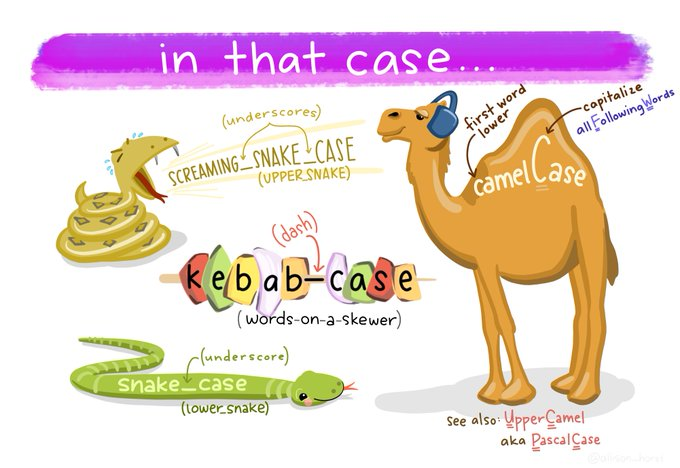
\includegraphics[width=\textwidth]{naming_conventions}
\caption{In Python ist \protect\say{Snake Case} üblich.\protect\footnotemark}
\label{figure-naming-conventions}
\end{figure}

\footnotetext{Bildquelle: \url{https://allisonhorst.com/everything-else}}